\chapter{Creating a Repository}
\label{sct:createrepo}

Though in principle a \cvmfs\ repository is just a directory tree, it is converted into a \newterm{repository} format first.
The repository format is in particular content addressable storage.
This task includes creating the file catalog(s), compressing the files and calculating content hashes.
Furthermore, we store the files in the same layout as the local \cvmfs\ cache on the server, \ie\ as SHA1 data chunks.
We do so to exploit redundancy and in order to mangle the real file name into an SHA1 key when \cvmfs\ downloads files.
This circumvents certain firewall restrictions.
For instance, many firewalls block an HTTP request to a file called \texttt{root.exe}.
Figure~\ref{fig:installwebserver} outlines the repository generation.

\begin{figure}[h]
	\begin{center}
		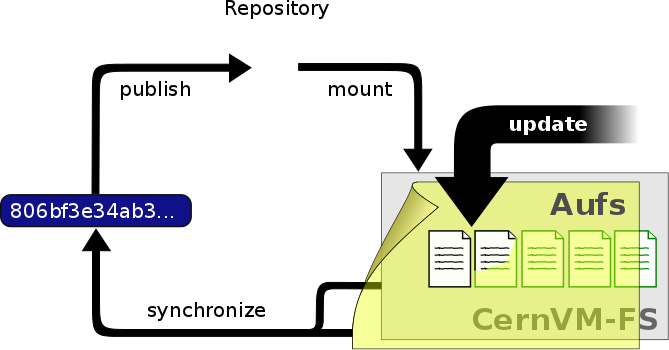
\includegraphics[width=0.8\textwidth]{figures/update_process}
	\end{center}
	\caption{Updating a mounted \cvmfs\ repository by overlaying it with a copy-on-write \aufs\ volume. Any changes will be accumulated in a writable volume (yellow) and can be synchronized into the file catalogs afterwards. The file catalog contains the directory structure as well as file metadata, symbolic links, and secure hash keys of regular files. Regular files are compressed and renamed to their cryptographic content hash before copied into the data store. (NOTE: bitmap will be replaced by vector graphic once I managed to export it)}
	\label{fig:installwebserver}
\end{figure}

\section{Repository Update Procedure}
\label{sct:repoupdate}

Since the repositories may contain many file system objects\footnote{For ATLAS, for example, ``many'' means order of $10^7$ file system objects (\ie number of regular files, symbolic links, and directories).}, we cannot afford to generate an entire repository from scratch for every update.
Instead, we add a writable file system layer on top of a mounted read-only \cvmfs\ repository using an union file system called \aufs~\cite{aufs}.
This renders a usual \cvmfs\ repository writable to the user, while all applied changes are stored in a special writable volume managed by \aufs.
One could see the result as a virtual version of the \emph{shadow tree} we used for updating repositories in previous versions of \cvmfs.
A similar approach is used by Linux Live Distributions that are shipped on read-only media, but allow \emph{virtual} editing of files while running the operating system directly from read-only storage.

If a file in the \cvmfs\ repository gets changed, \aufs\ first copies it to the writable volume and applies any changes to this copy (copy-on-write semantics).
\aufs\ will put newly created files or directories in the writable volume as well.
Additionally it creates special hidden files (called white-outs) to keep track of file deletions in the \cvmfs\ repository.

Eventually, all changes applied to the \emph{virtual shadow tree} are stored in \aufs's writable volume and can be merged into the actual \cvmfs\ repository by a subsequent synchronization step.
This includes compression of new and updated files and updating of the file catalogs.
Before the actual synchronization step takes place, no changes are applied to the \cvmfs\ repository itself.
Therefore, any unsuccessful updates to a repository can be rolled back by simply clearing the writable file system layer of \aufs.

\section{Requirements for a new Repository}
\label{sct:newreporequirements}

In order to create a repository, the server and client part of \cvmfs\ must be installed on your machine.
Furthermore your machine should provide an \aufs\ enabled Kernel as well as a running \texttt{Apache2} web server.
Currently we officially support Scientific Linux 5 and 6 as well as Ubuntu 12.04 distributions.
Please note, that Scientific Linux 6 \emph{does not} ship with an \aufs\ enabled kernel, therefore we provide a compatible patched kernel as an rpm (see Section~\ref{apx:rpms}).

Special care should be taken for the mount location of \cvmfs\ repositories.
From the point of view of the file system, repositories are relocatable.
However, many software installation tools hard-code the full path and therefore break relocatability on the application level.
In effect, repositories have to be mounted at the same location that was used to install it on the release manager machine.
By convention, \cvmfs\ repositories are mounted using their fully qualified repository name under \texttt{/cvmfs}, for instance at \texttt{/cvmfs/atlas.cern.ch}.

\section{\cvmfs\ Repository Creation and Updating}
\label{sct:repocreateandupdate}
To control the server part of \cvmfs\ we provide the versatile \texttt{cvmfs\_server} utility that controls repository creation, updating, deletion, replication and investigation.
Please run it without any parameters to get a short documentation of its commands.

\subsection{Repository Creation}
\label{sct:repocreation}

Given you have successfully installed the \cvmfs\ server part on your machine, you can use \texttt{cvmfs\_server mkfs} to create a fresh repository:\\
\texttt{cvmfs\_server mkfs my.repo.name}
The utility will then ask you for a user that should act as the owner of the repository and afterwards create all the infrastructure for your new \cvmfs\ repository.
Additionally it will create a reasonable default configuration and generate a new release manager certificate and software signing key. You should distribute the public key in \texttt{/etc/cvmfs/keys/my.repo.name} to all your client machines.
Please note, that the \texttt{cvmfs\_server} utility will use \texttt{/srv/cvmfs} as storage location.
In case you want to use a huge hard disk you should mount it there upfront.

When all went fine you should see your repository mounted under \texttt{/cvmfs/my.repo.name} containing only a single file called \texttt{new\_repository}.
Following this step, you can produce the first revision by going through the repository update procedure described in the next Section.

\subsection{Repository Update}
Typically a repository publisher does the following steps in order to create a new revision of a repository:
\begin{enumerate}
	\item Run \texttt{cvmfs\_server transaction} to switch to a copy-on-write enabled \cvmfs\ volume
	\item Make the necessary changes to the repository, \ie add new directories, patch certain binaries, \dots
	\item Test the software installation
	\item Do one of the following:
	\begin{itemize}
		\item Run \texttt{cvmfs\_server publish} and optionally \texttt{cvmfs\_server resign} to finalize your new repository revision \emph{or}
		\item Run \texttt{cvmfs\_server abort} to clear all changes and start over again
	\end{itemize}
	\item Make the web server serve the new version of the repository directory.
\end{enumerate}

Generally \cvmfs\ supports to have more than one repository on a single server machine, but then you need to specify which repository you want to operate on, when running the \texttt{cvmfs\_server} utility commands.
Additionally you should run \texttt{cvmfs\_server resign} every 30 days to update the signatures of the repository.
